\documentclass[10pt]{article}

\usepackage[T2A]{fontenc}
\usepackage[utf8x]{inputenc}

\usepackage[english,russian]{babel}
\usepackage{graphics, graphicx}

\usepackage{amsmath}
\usepackage{amssymb}
\usepackage{amsfonts}


\usepackage[left=20mm, top=20mm, right=20mm, bottom=20mm, nohead, nofoot, footskip=15pt]{geometry}

\usepackage{color}
\usepackage{epsfig}
\usepackage{bm}
\usepackage[colorlinks,urlcolor=blue]{hyperref}
\usepackage{tikz}
\usepackage{pgfplots}



\tolerance=1
\emergencystretch=\maxdimen
\hyphenpenalty=10000
\hbadness=10000


\author{Дмитриев Леонид, группа 317}

\title{
	Обработка и распознавание изображений\\
	Лабораторная работа № 2\\
	Изучение и освоение методов классификации формы изображений
}

\begin{document}
	{
		\LARGE
		\maketitle
	}
	
	\clearpage
	
	
	{ \large \tableofcontents} 
	
	\clearpage
	
	
	
	\section*{Постановка задачи}
	\addcontentsline{toc}{section}{Постановка задачи}
	
	\large
	
	
	Целью работы является разработка и реализация программы для классификации изображений моделей графов,
	построенных из магнитной головоломки.\\
	Программа должна обеспечивать:
	\begin{itemize}
		\item Ввод и отображение на экране изображений в формате JPEG
		
		\item Сегментацию изображений на основе точечных и пространственных преобразований
		
		\item Генерацию признаковых описаний структуры графов на изображении
		
		\item Классификацию изображений по 4 заданным классам
	\end{itemize}
	
	Задание делится на два вида сложности (Intermediate и Expert). В первом случае фон белый, а во втором пестрый.
	
	
	\section*{Описание данных}
	\addcontentsline{toc}{section}{Описание данных}
	
	Входными данными являются цветные изображения моделей, из деталей магнитной игры - головоломки в формате $1024 \times 768$ с разрешением 72 dpi.
	
	Всего задано 4 структуры графов, эталоны которых представлены на 4 имеющихся изображениях.
	
	\begin{figure}[h]
		\begin{minipage}[h]{0.45\linewidth}
			\begin{center}
				{\includegraphics[width=1.0\linewidth]{data/2.pdf}}
			\end{center}
		\end{minipage}
		\hfill
		\begin{minipage}[h]{0.45\linewidth}
			\begin{center}
				{\includegraphics[width=1.0\linewidth]{data/3.pdf}}
			\end{center}
		\end{minipage}
		\vfill
		\begin{minipage}[h]{0.45\linewidth}
			\begin{center}
				{\includegraphics[width=1.0\linewidth]{data/4.pdf}}
			\end{center}
		\end{minipage}
		\hfill
		\begin{minipage}[h]{0.45\linewidth}
			\begin{center}
				{\includegraphics[width=1.0\linewidth]{data/5.pdf}}
			\end{center}
		\end{minipage}
		\caption{Изображения эталонов 4 типов графов.}
		\label{ris:image1}
	\end{figure}

	На остальных изображениях представлены графы, изоморфные 4 эталонным образцам. При этом вершинами считаются только узлы степени не равной 2 и длины ребер (веса) не учитываются.
	
	\begin{figure}[h]
		\begin{center}
			{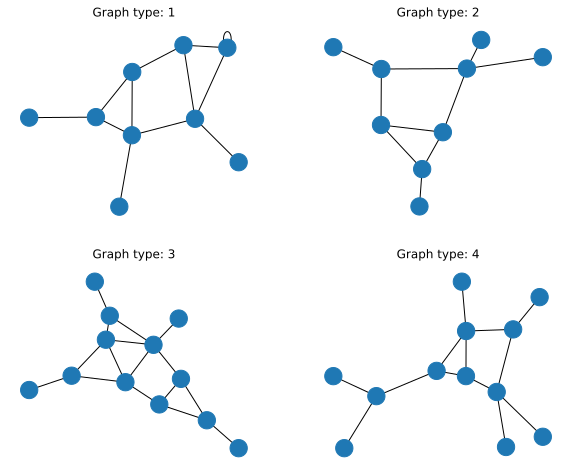
\includegraphics[width=0.68\linewidth]{data/graph_types.pdf}}
		\end{center}
		\caption{Изображения типов структур графов.}
		\label{ris:image2}
	\end{figure}
	
	Для задачи повышенной сложности фон на изображениях разноцветный и с множеством прямых линий.
	
	\begin{figure}[h]
		\begin{minipage}[h]{0.45\linewidth}
			\begin{center}
				{\includegraphics[width=1.0\linewidth]{data/9.pdf}}
			\end{center}
		\end{minipage}
		\hfill
		\begin{minipage}[h]{0.45\linewidth}
			\begin{center}
				{\includegraphics[width=1.0\linewidth]{data/16.pdf}}
			\end{center}
		\end{minipage}
		\caption{Примеры изображений повышенной сложности.}
		\label{ris:image3}
	\end{figure}
	
	
	\section*{Описание метода решения}
	\addcontentsline{toc}{section}{Описание метода решения}
	
	Этапы извлечения графа из изображения:
	\begin{itemize}
		\item Сегментация графа, переход к бинарному изображению
		\item Построение скелета графа
		\item Извлечение из скелета графа вершин и ребер, построение программной модели графа
		\item Извлечение из структуры графа вектора признаков
		\item Классификация графа по имеющимся признакам
	\end{itemize}
	
	\subsection*{Сегментация графа, получение бинарного изображения}
	\addcontentsline{toc}{subsection}{Сегментация графа, получение бинарного изображения}
	
	Для обоих уровней сложности реализованы похожие методы решения. Единственным различием является этап бинаризации.
	
	\subsubsection*{Intermediate}
	\addcontentsline{toc}{subsubsection}{Intermediate}
	
	Сперва из изображения устраняется шум. Для этого применяется медианная свёртка.
	
	\begin{figure}[h]
		\begin{minipage}[h]{0.4\linewidth}
			\begin{center}
				{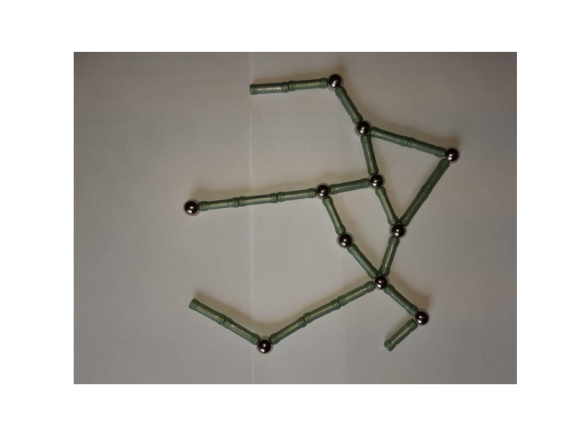
\includegraphics[width=1.0\linewidth]{data/median_blur_start.pdf}}
			\end{center}
		\end{minipage}
		\hfill
		\begin{minipage}[h]{0.4\linewidth}
			\begin{center}
				{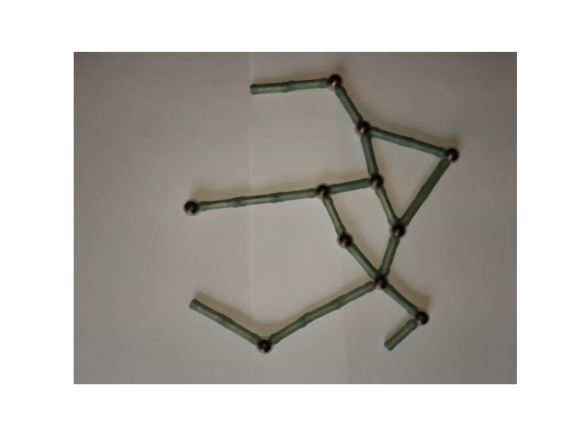
\includegraphics[width=1.0\linewidth]{data/median_blur.pdf}}
			\end{center}
		\end{minipage}
		
		\caption{Исходник (слева), результат медианной свёртки (справа).}
		\label{ris:image4}
	\end{figure}
	
	Убирать шум необходимо для лучшего обнаружения краев с помощью свертки (функция Canny из библиотеки OpenCV). Также сразу отсекаются по порогам шумовые пиксели, не являющиеся предметами интереса.
	
	Для построения скелета необходимо залить объект, это можно сделать с помощью операции закрытия с большой матрицей свёртки.
	
	\begin{figure}[h]
			\begin{minipage}[h]{0.36\linewidth}
					{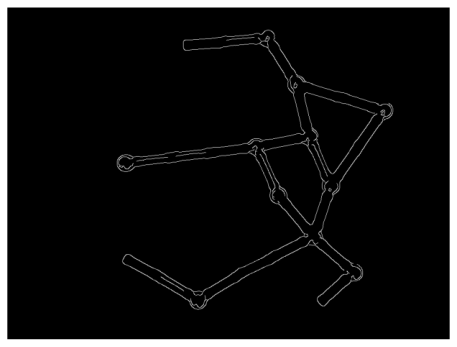
\includegraphics[width=1.0\linewidth]{data/edges.pdf}}
			\end{minipage}
		\hfill
			\begin{minipage}[h]{0.36\linewidth}
				{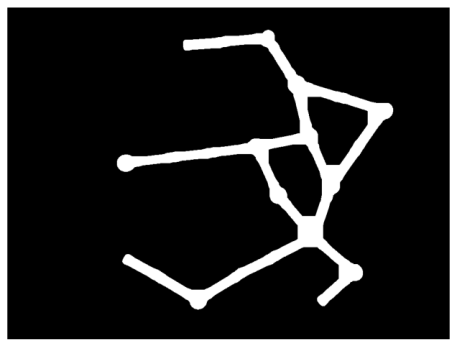
\includegraphics[width=1.0\linewidth]{data/inter_bin.pdf}}
			\end{minipage}
		
		\caption{Результаты обнаружения краёв (слева) и применения закрытия к обнаруженным краям (справа).}
		\label{ris:image5}
	\end{figure}
	
	
	
	\subsubsection*{Expert}
	\addcontentsline{toc}{subsubsection}{Expert}
	
	Сначала изображение переводится в HSV формат, а затем с помощью нескольких масок диапазонов значений сегментируются ребра и вершины по отдельности, после этого маски складываются.
	
	\begin{figure}[h]
		\begin{minipage}[h]{0.3\linewidth}
			\begin{center}
				{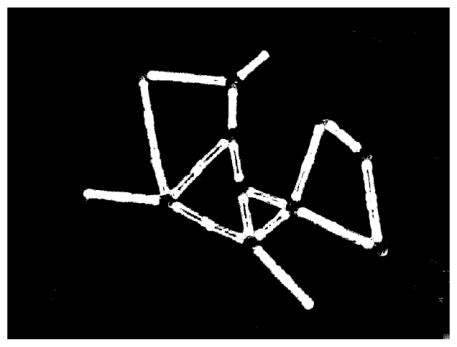
\includegraphics[width=1.0\linewidth]{data/expert_green.pdf}}
			\end{center}
		\end{minipage}
		\hfill
		\begin{minipage}[h]{0.3\linewidth}
			\begin{center}
				{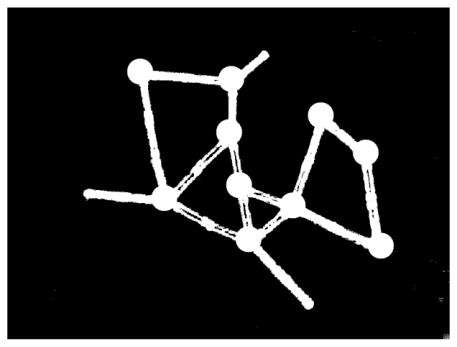
\includegraphics[width=1.0\linewidth]{data/expert_with_circles.pdf}}
			\end{center}
		\end{minipage}
		
		\caption{Результат детектирования ребер и вершин.}
		\label{ris:image6}
	\end{figure}
	
	
	Далее удаляется шум с помощью открытия, а затем устраняются внутренние полости с помощью закрытия.
	
	\begin{figure}[h]
		\begin{minipage}[h]{0.3\linewidth}
			\begin{center}
				{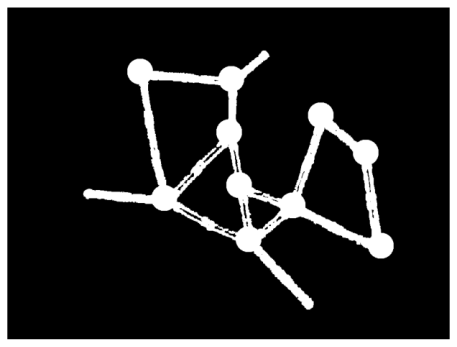
\includegraphics[width=1.0\linewidth]{data/expert_del_noise.pdf}}
			\end{center}
		\end{minipage}
		\hfill
		\begin{minipage}[h]{0.3\linewidth}
			\begin{center}
				{\includegraphics[width=1.0\linewidth]{data/expert_bin.pdf}}
			\end{center}
		\end{minipage}
		
		\caption{Результаты удаления шума и удаления полостей.}
		\label{ris:image7}
	\end{figure}
	
	
	\subsection*{Построение скелета}
	\addcontentsline{toc}{subsection}{Построение скелета}
	
	
	Скелет изображения строится по алгоритму Розенфельда (функция skeletonize из библиотеки skimage).
	
	\begin{figure}[h]
		\begin{center}
			{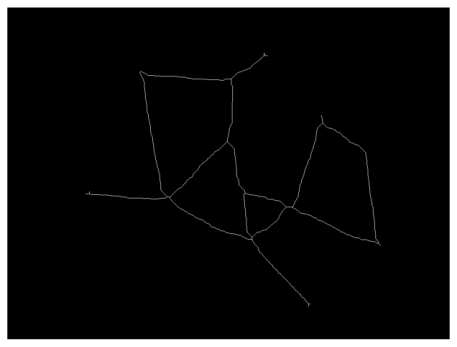
\includegraphics[width=0.4\linewidth]{data/skeleton.pdf}}
		\end{center}
		\caption{Пример скелета графа изображения.}
		\label{ris:image8}
	\end{figure}
	
	
	
	\subsection*{Извлечение из скелета графа вершин и ребер, построение программной модели графа}
	\addcontentsline{toc}{subsection}{Извлечение из скелета графа вершин и ребер, построение программной модели графа}
	
	Была реализована программа по извлечению графа из изображения скелета. Так как функция skeletonize использует специфичный тип соседства пикселей было введено специальное правило определения связи между пикселями.
	
	Сильными связями считаются связи по горизонтали и вертикали, если такая связь есть то она учитывается всегда. Слабыми связями считаются связи по диагоналям, такая связь учитывается только если нет обеих прилегающих к этому месту сильных связей.
	
	Реализованный алгоритм возвращает все найденные компоненты связности на изображении в виде графов (множеств из вершин и ребер).
	
	\begin{figure}[h]
	\begin{minipage}[h]{0.4\linewidth}
		\begin{center}
			{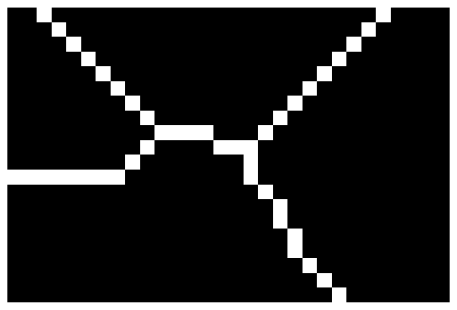
\includegraphics[width=1.0\linewidth]{data/crop_1.pdf}}
		\end{center}
	\end{minipage}
	\hfill
	\begin{minipage}[h]{0.4\linewidth}
		\begin{center}
			{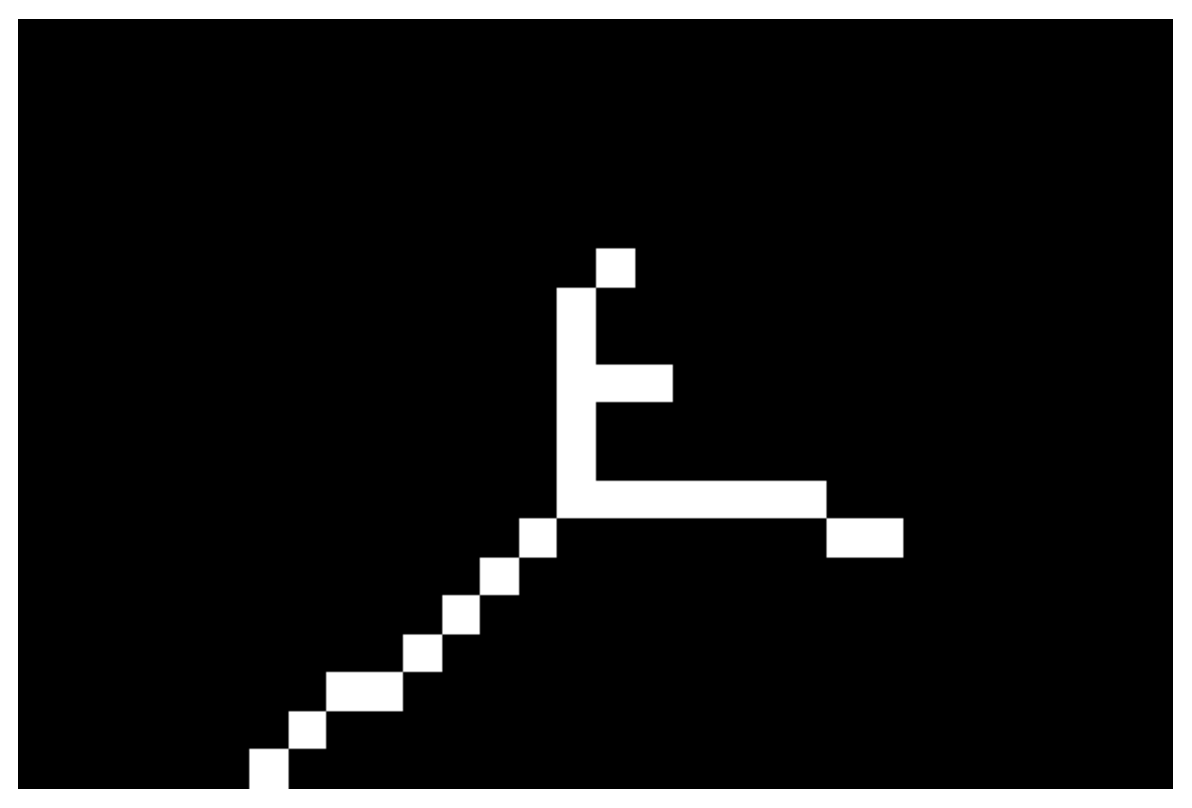
\includegraphics[width=1.0\linewidth]{data/crop_2.pdf}}
		\end{center}
	\end{minipage}
	
		\caption{Пример типичной вершины со степенью 4(слева), пример шумовых ветвей(справа).}
		\label{ris:image9}
	\end{figure}
	
	Но в итоге построенный граф не является структурно в точности таким же, как на исходном изображении. Это вызвано тем, что при получении скелета происходит расщепление вершин большой степени и появлении мелких шумовых ветвей (показано на рисунке выше). Данная проблема решается поочередным применением операции удаления короткого терминального ребра и операции склеивания вершин связанных коротким ребром. Операции продолжаются до тех пор, пока существуют короткие ребра (короткий - значит длина меньше порога).
	
	
	\begin{figure}[h]
		\begin{center}
			{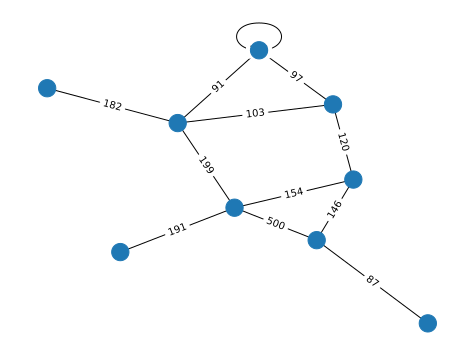
\includegraphics[width=0.5\linewidth]{data/graph_example.pdf}}
		\end{center}
		\caption{Пример программной модели.}
		\label{ris:image10}
	\end{figure}
	
	
	\subsection*{Извлечение из структуры графа вектора признаков}
	\addcontentsline{toc}{subsection}{Извлечение из структуры графа вектора признаков}
	
	Из графа извлекаются следующие признаки: число ребер, число вершин, число терминальных вершин со степенью 1, число вершин со степенью 3, число вершин со степенью 4, число вершин со степенью 5, число циклов в базисе, число петель, число внутренних ребер, кол-во циклов содержащих три вершины.
	
	Для графа разобранного выше (в expert бинаризации) вектор признаков равен:\\
	\[12, 9, 3, 3, 3, 0, 4, 1, 9, 2\].
	
	\begin{itemize}
		\item Для класса 1: [12  9  3  3  3  0  4  1  9  2]
		\item Для класса 2: [10  9  4  4  1  0  2  0  6  1]
		\item Для класса 3: [16 12  4  5  2  1  5  0 12  4]
		\item Для класса 4: [13 12  6  4  2  0  2  0  7  1]
	\end{itemize}
	
	
	
	\subsection*{Классификация графа по имеющимся признакам}
	\addcontentsline{toc}{subsection}{Классификация графа по имеющимся признакам}
	
	Сначала производится попытка проверить изоморфизм полученного графа со всеми заранее найденными эталонными графами, если при построении графа не произошло ошибок, то будет найден верный класс.
	
	Если класс не был найден, то произошла и дальше действуем из предположения, что вектор признаков полученный ранее должен быть ближе всего к вектору признаков верного класса. Таким образом выбираем наиболее близкий класс. 
	
	Выбор класса по близости производится с помощью логистической регрессии обученной на 4 эталонных графах, где векторы признаков нормализуются. Этот способ выбран так как линейная модель нативно оценивает важность признаков.
	
	
	\section*{Описание программной реализации}
	\addcontentsline{toc}{section}{Описание программной реализации}
	
	Программная реализация оформлена в виде юпитер-ноутбука program.ipynb,
	в котором объявляются переменные FILENAME и TASK\_TYPE.
	
	FILENAME - необходимо присвоить ей значение имени файла с входным изображением.
	
    
    Для выполнения решения для задачи Intermediate:
    
	TASK\_TYPE = "inter"
	
	Для выполнения решения для задачи Expert:
	
	TASK\_TYPE = "expert"
	
	
	После присвоения соответствующих значений необходимо выполнить все строчки кода ноутбука с первой до последней, в итоге в предпоследней ячейке будет напечатан класс входного графа.
	
	
	\section*{Эксперименты}
	\addcontentsline{toc}{section}{Эксперименты}
	
	При проверке на всех тренировочных изображениях алгоритм корректно определял тип входного графа.
	
	\section*{Выводы}
	\addcontentsline{toc}{section}{Выводы}
	
	Была разработана и реализована программа, определяющая по входному изображению тип графа расположенного на нем среди заданных 4 классов. 
	
	
\end{document}
